% !TeX root = ../../Book5.tex
% 纲要标题：### 1.5 模型提出的结构问题
% 纲要位置：几何学计划纲要.md，第 5062 行。
% 正文状态：初稿；尚未正式审核。

% 纲要内容开始
% 
% * 结点、尖点与非约化点
% * 射影闭包中的无穷远分支
% * 为什么必须保留局部环和概形纤维
% 
% ---
% 
% 纲要内容结束

\section{模型提出的结构问题}
\label{g5:sec:0105}

消去给出映射像的闭包，参数化给出函数域，射影闭包补入无穷远点。这几种构造保留的信息不同。下面比较两个有理三次曲线，并考察两点重合时的方程；计算将说明，研究一个点附近的函数及保留方程中的幂次，怎样补充点集和函数域的描述。

\subsection{结点、尖点与非约化点}
\label{g5:subsec:0105:01}

先设 \(k\) 为代数闭域且 \(\operatorname{char}k\ne2\)，考虑
\[
	C_{\mathrm n}=V(y^2-x^2(x+1)),\qquad
	C_{\mathrm c}=V(y^2-x^3).
\]
第二条是\cref{g5:exm:cusp-birational}的尖点曲线。第一条曲线可用过原点的直线 \(y=tx\) 求参数：代入并取 \(x\ne0\)，得到
\[
	x=t^2-1,\qquad y=t(t^2-1).
\]
由此定义正则映射
\[
	\nu_{\mathrm n}:\mathbb A_k^1\longrightarrow C_{\mathrm n},
	\qquad t\longmapsto(t^2-1,t(t^2-1)).
\]
在 \(x\ne0\) 处，逆参数是 \(t=y/x\)；原点则有两个参数原像 \(t=1,-1\)。其坐标环确实为 \(k[t^2-1,t(t^2-1)]\)：将多项式除以关于 \(y\) 首一的方程后，余式为 \(a(x)+yb(x)\)。代入参数，第一项是 \(t\) 的偶多项式，第二项是奇多项式；两者之和为零迫使两者都为零，并进而迫使 \(a=b=0\)。所以代入同态的核恰好为所给主理想，它为素理想，曲线因而不可约。

\ProseParagraphBreak

在原点平移展开方程，最低次非零齐次项分别为
\[
	y^2-x^2=(y-x)(y+x),\qquad y^2.
\]
把最低次非零齐次方程给出的锥连同因子重数，称为这个平面曲线模型的\term[qiezhui]{切锥}[tangent cone]，第一式给两个不同方向，第二式给同一方向的二重方程。这里的两个方向还可以从参数的局部变化看出：在 \(t=1\) 附近令 \(t=1+s\)，则 \(x=2s+s^2\)、\(y=2s+3s^2+s^3\)；在 \(t=-1\) 附近令 \(t=-1+s\)，则 \(x=-2s+s^2\)、\(y=2s-3s^2+s^3\)。它们分别有方向 \(y=x\)、\(y=-x\)。这种模型的原点称为\term[jiedian]{结点}[node]；\(C_{\mathrm c}\) 的原点称为\term[jiandian]{尖点}[cusp]。参数化的比较也可参见\cite[第I章第4节，例4.9.1及习题4.10]{Hartshorne1977}。

\ProseParagraphBreak

在 \(k=\mathbb C\) 时，\cref{g5:fig:node-cusp}画出实参数所描绘的实点截面。结点的两个参数值对应同一个平面点，尖点则由一个参数值产生；完整的局部区分由随后的方程计算给出。
\begin{figure}[htbp]
	\centering
	% !TeX root = ../Book5.tex
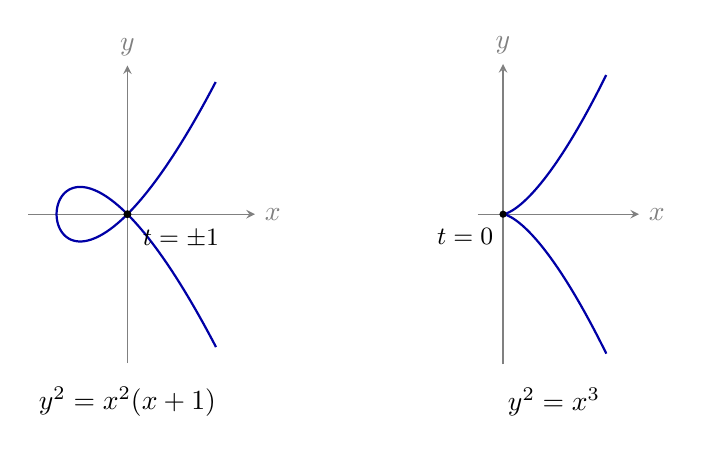
\begin{tikzpicture}[>=stealth,scale=.9]
	\begin{scope}[xshift=0cm]
		\draw[->,gray] (-1.4,0)--(1.8,0) node[right]{\(x\)};
		\draw[->,gray] (0,-2.1)--(0,2.1) node[above]{\(y\)};
		\draw[thick,blue!65!black,domain=-1.5:1.5,samples=151,variable=\t]
			plot ({\t*\t-1},{\t*(\t*\t-1)});
		\fill (0,0) circle (1.6pt);
		\node[below right,font=\small] at (.08,-.08){\(t=\pm1\)};
		\node at (0,-2.65){\(y^2=x^2(x+1)\)};
	\end{scope}
	\begin{scope}[xshift=5.3cm,scale=.8]
		\draw[->,gray] (-.45,0)--(2.4,0) node[right]{\(x\)};
		\draw[->,gray] (0,-2.65)--(0,2.65) node[above]{\(y\)};
		\draw[thick,blue!65!black,domain=-1.35:1.35,samples=121,variable=\t]
			plot ({\t*\t},{\t*\t*\t});
		\fill (0,0) circle (1.8pt);
		\node[below left,font=\small] at (0,-.08){\(t=0\)};
		\node at (.9,-3.31){\(y^2=x^3\)};
	\end{scope}
\end{tikzpicture}

	\caption[结点与尖点的参数模型]{结点与尖点的实点截面。左图参数为 \((t^2-1,t(t^2-1))\)，右图参数为 \((t^2,t^3)\)。}
	\label{g5:fig:node-cusp}
\end{figure}
全局不可约曲线也能在一个点有两个局部分支。为把上面的说法落实到方程，可以允许形式幂级数，即按总次数逐项运算、不讨论数值收敛的级数。在 \(k[[x]]\) 中，方程 \(s(x)^2=1+x\)、\(s(0)=1\) 有唯一解：若 \(s=1+\sum_{r\ge1}c_rx^r\)，逐次比较系数给出
\[
	2c_r=\delta_{r1}-\sum_{i=1}^{r-1}c_i c_{r-i}.
\]
特征不为二保证每步可解。因此在 \(k[[x,y]]\) 中，
\[
	y^2-x^2(x+1)=(y-xs(x))(y+xs(x)).
\]
两个因子分别给出形式图像 \(y=\pm xs(x)\)，每个图像的商环同构于 \(k[[x]]\)，两个因子不是彼此的单位倍。这具体显示了两条形式分支，尽管多项式坐标环本身是整环。

\ProseParagraphBreak

尖点的形式方程则仍不可约。代入 \(x=t^2,y=t^3\) 将
\(k[[x,y]]/(y^2-x^3)\) 嵌入 \(k[[t]]\)：利用 \(y^2=x^3\)，每个类都可唯一写成 \(a(x)+yb(x)\)，其中 \(a,b\in k[[x]]\)。这一归约对幂级数有意义，因为把 \(y^{2r}\) 换成 \(x^{3r}\) 后，对任一固定次数只有有限项贡献。代入后偶次幂与大于等于三的奇次幂不相混，故核为零。商环是整环，因而形式方程有一条分支。这里把形式方程的不可约因子所确定的部分称为形式分支；一般局部环与其完备化的关系将在后续章节系统建立。

\begin{example}\label{g5:exm:nonreduced-point}
	在任意代数闭域 \(k\) 上，方程 \(x=0\) 与 \(x^2=0\) 有同一零点集，商环却分别为
	\[
		k[x]/(x)\simeq k,\qquad
		k[x]/(x^2)\simeq k[\varepsilon]/(\varepsilon^2).
	\]
	后一个环中 \(\varepsilon\ne0\) 而 \(\varepsilon^2=0\)。环中某个正整数次幂为零的元素称为幂零元；没有非零幂零元的环称为约化环。前者是一个约化点的函数环，后者是一个\term[feiyuehuadian]{非约化点}[nonreduced point]的代数模型。作为 \(k\) 向量空间，它们的维数分别为一和二，后一空间的基为 \(1,\varepsilon\)。

	每个到 \(k\) 的 \(k\) 代数同态都把 \(\varepsilon\) 送到零，因而普通 \(k\) 值点看不到这个区别。若允许取值于 \(D=k[\varepsilon]/(\varepsilon^2)\)，则把坐标 \(x\) 送到 \(a\varepsilon\)（\(a\in k\)）都满足 \(x^2=0\)，却只有 \(a=0\) 满足 \(x=0\)。保留这些测试环中的解，就能检测点集中消失的信息。
\end{example}

\subsection{射影闭包中的无穷远分支}
\label{g5:subsec:0105:02}

在 \(\mathbb P_k^2\) 中使用坐标 \([X:Y:Z]\)，把 \(Z\ne0\) 作为原仿射平面。前面两条曲线的射影闭包为
\[
	\overline C_{\mathrm n}=V_+(Y^2Z-X^2(X+Z)),\qquad
	\overline C_{\mathrm c}=V_+(Y^2Z-X^3).
\]
两者在 \(Z=0\) 上都只有 \(P_\infty=[0:1:0]\)。在 \(Y\ne0\) 的图上令 \(u=X/Y,v=Z/Y\)，方程变成
\[
	v-u^3-u^2v=0,\qquad v-u^3=0.
\]
结点模型中 \(1-u^2\) 在 \(P_\infty\) 附近不为零，所以 \(v=u^3/(1-u^2)\)；尖点模型中 \(v=u^3\)。每个模型在无穷远点附近都由一个正则参数 \(u\) 描述，只有一条这样的局部分支。

\ProseParagraphBreak

这也可由射影参数直接核验。将仿射参数写成 \(t=T/S\)，得到
\[
\begin{aligned}
	\nu_{\mathrm n}([S:T])
		&=[S(T^2-S^2):T(T^2-S^2):S^3],\\
	\nu_{\mathrm c}([S:T])
		&=[ST^2:T^3:S^3].
\end{aligned}
\]
两组坐标均为同次齐次多项式，而且在 \(\mathbb P^1\) 上没有公共零点：\(S\ne0\) 时最后一个坐标非零，\(S=0\) 时第二个坐标非零。代入曲线方程检验像确实落在闭包内，且 \(S=0\) 唯一地映到 \(P_\infty\)。这些射影像包含原仿射曲线及其无穷远点，故给出了闭包的全部点。

\begin{example}\label{g5:exm:two-infinity-branches}
	双曲线 \(xy=1\) 的射影闭包为 \(XY=Z^2\)，有两个无穷远点 \([1:0:0]\)、\([0:1:0]\)。在第一点附近用 \(u=Y/X,v=Z/X\)，方程为 \(u=v^2\)；另一点同理。两个点附近各有一条参数分支。参数 \(x=t,y=t^{-1}\) 中的 \(t=0\) 与 \(t=\infty\) 在射影闭包中成为两个不同点。
\end{example}

无穷远点的个数与局部分支的个数须分别判断。把一个结点移到无穷远处即可看到差别：在 \(\overline C_{\mathrm n}\) 中改以直线 \(X=0\) 为无穷远直线，原结点 \([0:0:1]\) 就成为无穷远点，仍带有两条形式分支。由此，齐次化后列出无穷远点只是第一步；还需要在各点的仿射图内查看方程或参数。

\subsection{为什么必须保留局部环和概形纤维}
\label{g5:subsec:0105:03}

一个有理函数能否在指定点延拓，取决于该点附近能否找到不消失的分母。为了把所有这样的函数放在同一对象中，设 \(X\) 为仿射代数集，\(p\in X\)。把包含 \(p\) 的开邻域 \(U\) 上的正则函数 \(f\) 与另一个 \((V,g)\) 视为相同，只要两者在某个更小的 \(p\) 的邻域上相等。所得等价类称为函数在 \(p\) 的\term[hanshuya]{芽}[germ]，其环记为
\[
	\mathcal O_{X,p}=\{\text{在 }p\text{ 附近的正则函数芽}\}.
\]
\symidx{\(\mathcal O_{X,p}\)：\(X\) 在 \(p\) 处的局部环}

\begin{proposition}\label{g5:prop:model-local-ring}
	设 \(k\) 为代数闭域，\(X\) 为仿射代数集，\(p\in X\)，\(A=k[X]\)。每个函数芽都可写成 \(a/b\)，其中 \(a,b\in A\)、\(b(p)\ne0\)。两个这样的分式代表同一芽，当且仅当存在 \(h\in A\)、\(h(p)\ne0\)，使
	\[
		h(ad-bc)=0
	\]
	成立，其中所比较的分式为 \(a/b\) 与 \(c/d\)。此环有唯一极大理想
	\[
		\mathfrak m_p=\{f\in\mathcal O_{X,p}:f(p)=0\},
		\qquad \mathcal O_{X,p}/\mathfrak m_p\simeq k.
	\]
\end{proposition}
\begin{proof}
	分式表达来自正则函数的定义。若两分式在一个邻域内相等，取包含 \(p\) 并位于该邻域内的主开集 \(D(h)\)。函数 \(ad-bc\) 在 \(D(h)\) 上为零，所以 \(h(ad-bc)\) 在整个 \(X\) 上为零。反之，上述等式在 \(D(hbd)\) 上可以除以不消失的分母，给出分式相等。

	求值到 \(k\) 是满同态，其核即 \(\mathfrak m_p\)，因此它是极大理想。若 \(f(p)\ne0\)，在较小邻域上 \(1/f\) 正则，所以 \(f\) 是单位；若 \(f(p)=0\)，求值表明它不可能为单位。因此所有非单位恰组成 \(\mathfrak m_p\)，任何真理想都包含在其中，极大理想唯一。
\end{proof}

只有一个极大理想的交换环称为\term[jubuhuan]{局部环}[local ring]。命题给出的分式环就是记号 \(A_{\mathfrak m}\) 所表示的局部化，其中 \(\mathfrak m=\{a\in A:a(p)=0\}\)。\cref{g5:exm:cusp-local-obstruction}证明了尖点处的局部环不含函数 \(t=y/x\)，而参数直线原点的局部环含有它；局部环由此记录了双有理对应中被遗漏的差别。

\ProseParagraphBreak

一阶测试可以同时检测局部函数及非约化信息。设 \(A=k[x_1,\ldots,x_n]/I\)，并固定一个零点 \(p=(p_1,\ldots,p_n)\)。到双数环 \(D=k[\varepsilon]/(\varepsilon^2)\) 的同态，若模 \(\varepsilon\) 后等于在 \(p\) 的求值，必把坐标送到
\[
	x_i\longmapsto p_i+v_i\varepsilon .
\]
对任意 \(F\in I\)，直接展开每个单项式得到
\[
	F(p+v\varepsilon)=F(p)+
	\varepsilon\sum_{i=1}^n\frac{\partial F}{\partial x_i}(p)v_i.
\]
因而这个赋值能通过商环，当且仅当每个 \(F\in I\) 的一次项都为零。这一解空间是该方程模型在 \(p\) 的\term[Zariskiqiekongjian]{Zariski 切空间}[Zariski tangent space]。计算时只需检查理想生成元：对 \(F=\sum_j a_jF_j\)，因 \(F_j(p)=0\)，一次项就是各 \(F_j\) 一次项的 \(a_j(p)\) 倍之和。

\ProseParagraphBreak

在结点和尖点原点，两方程的一次项都为零，故两者的切空间都是 \(k^2\)；切锥又分别保留了两个方向和一个二重方向。对约化点 \(A=k[x]/(x)\)，一次项条件为 \(v=0\)；对 \(A=k[x]/(x^2)\)，一次项没有约束，得到一维切空间。可见一阶线性化、最低次方程和完整局部环各自保留不同层次的信息。

\begin{example}\label{g5:exm:double-cover-fibres}
	设 \(k\) 为代数闭域且 \(\operatorname{char}k\ne2\)。考虑映射
	\[
		\pi:\mathbb A_k^1\longrightarrow\mathbb A_k^1,\qquad t\longmapsto s=t^2.
	\]
	在 \(s=a\) 上的集合论纤维是方程 \(t^2=a\) 的根集。若直接在坐标环中加入基底方程 \(s-a=0\)，得到纤维代数
	\[
		B_a=k[t]/(t^2-a).
	\]
	当 \(a=b^2\ne0\) 时，\(b\ne-b\)，求值给出同构
	\[
		B_a\longrightarrow k\times k,\qquad f\longmapsto(f(b),f(-b)).
	\]
	其核由 \((t-b)(t+b)\) 生成，满射性可用插值多项式 \((t+b)/(2b)\)、\((b-t)/(2b)\) 核验。当 \(a=0\) 时，
	\(B_0=k[t]/(t^2)\)，有一个二重点。每个 \(B_a\) 都有向量空间基 \(1,t\)，维数恒为二；只取根集，则点数从二变为一。

	特征条件在这里有直接作用：若 \(\operatorname{char}k=2\)，每个 \(a=b^2\) 都满足 \(t^2-a=(t-b)^2\)，所有纤维代数都有非零幂零元。
\end{example}

一般地，若映射由 \(k[s_1,\ldots,s_m]\rightarrow B\)、\(s_i\mapsto f_i\) 给出，在指定点 \(a=(a_1,\ldots,a_m)\) 上保留方程的纤维代数是
\[
	B/(f_1-a_1,\ldots,f_m-a_m).
\]
它满足明确的映射性质：对于任意 \(k\) 代数 \(R\)，从此商环到 \(R\) 的同态，恰对应从 \(B\) 到 \(R\) 且把每个 \(f_i\) 送到 \(a_i\) 的同态。这正是“在基底点上取纤维”对各种测试环应有的含义。把纤维理想替换为其根式再取商，只保留约化的点集结构，会丢掉\cref{g5:exm:double-cover-fibres}中的二重结构。

\ProseParagraphBreak

概形将允许非约化的交换环作为仿射模型，并把这些环的局部信息粘合起来；以上商环随后会成为仿射概形纤维的坐标环。接下来的局部化、有限模与整性理论，分别用于组织点附近的函数、控制代数的有限性，以及比较原曲线和参数曲线。此处各个模型已经显示了这些构造要保留的具体信息。
